\section{Diagrama de Sequência}
O diagrama de sequência é uma representação gráfica que descreve como objetos interagem em um cenário específico, mostrando a ordem das mensagens trocadas entre eles ao longo do tempo. Utilizado na modelagem de comportamento, ele ajuda a visualizar a dinâmica do fluxo de controle e comunicação em um sistema.


\subsection{Diagrama de Sequencia Gerenciar Eventos}

Na Figura \ref{fig:19} o administrador gerencie a agenda do escritório por meio de um calendário interativo:

\begin{itemize} \item Ao acessar a página inicial, o calendário é carregado com todos os eventos armazenados no banco de dados. \item O administrador pode adicionar novos eventos preenchendo um formulário com informações como título, data, descrição e cor. \item Eventos existentes podem ser editados diretamente via um modal interativo, com atualizações sendo salvas por requisições AJAX. \item A exclusão de eventos também ocorre via modal, com confirmação e remoção imediata do calendário. \end{itemize}
Esse fluxo é dinamicamente atualizado no frontend com o uso da biblioteca \texttt{FullCalendar}, mantendo a sincronização com os dados persistidos no backend.


\subsection{Diagrama de Sequencia Marcar Consulta}

Na Figura \ref{fig:20} o cliente agenda consultas jurídicas por meio de um formulário interativo:

\begin{itemize} \item Ao acessar a página, o cliente visualiza um formulário e uma tabela com suas consultas já marcadas. \item Ao selecionar uma data, o sistema consulta os horários disponíveis para aquele dia, excluindo os já ocupados. \item O cliente escolhe o horário e preenche as informações da consulta, que é registrada no sistema após envio do formulário. \item A consulta recém-criada aparece na lista do cliente e os horários são atualizados dinamicamente. \item O cliente também pode excluir consultas anteriores, com a atualização automática da agenda. 
\end{itemize}
Esse fluxo garante controle total do agendamento por parte do cliente, com sincronização em tempo real via AJAX.

\subsection{Diagrama de Sequencia Gerenciar Pagamento}

Na Figura \ref{fig:21} o administrador gere cobranças via QR Code PIX, mesmo para clientes que não estão cadastrados no sistema:

\begin{itemize} \item O administrador acessa a interface de geração de PIX e visualiza um formulário para inserção do nome do cliente e valor a ser cobrado. \item Após o envio do formulário, o sistema gera automaticamente o payload PIX e seu respectivo QR Code utilizando a biblioteca \texttt{BaconQrCode}. \item A transação gerada é registrada no banco de dados e adicionada à lista de histórico visível na mesma página. \item O administrador pode também excluir transações anteriores diretamente da lista, com atualização imediata da interface. \end{itemize}
Este fluxo permite manter um controle prático e histórico de cobranças avulsas, sem necessidade de vínculo direto com um usuário autenticado.

\subsection{Diagrama de Sequencia Processar Pagamento}

Na Figura \ref{fig:22} o cliente visualize e pague suas parcelas pendentes referentes ao mês atual:

\begin{itemize} \item Ao acessar a página de pagamento, o sistema filtra e exibe apenas as parcelas pendentes do cliente no mês vigente. \item Para cada parcela exibida, o cliente pode clicar em "Gerar Pagamento", acionando a geração de um QR Code PIX. \item O sistema valida a autorização de acesso à parcela, gera o payload conforme o padrão Pix e exibe o QR Code para pagamento. \item O cliente deve então realizar o pagamento manualmente usando seu aplicativo bancário. \item Após o pagamento, o administrador deve confirmar manualmente no sistema através da funcionalidade \textit{Gerenciar Recursos Financeiros}. \end{itemize}

Este fluxo não possui automação de confirmação de pagamento, funcionando com validação visual por parte do administrador.

\subsection{Diagrama de Sequencia Acompanhar Processo Jurídico}

Na Figura \ref{fig:23} o cliente pode consultar o andamento de seus processos jurídicos cadastrados no sistema:

\begin{itemize} \item O cliente acessa a página de processos, onde é exibida uma lista com todos os processos atribuídos a ele, incluindo número, descrição, status atual e data da última atualização. \item Ao clicar em "Ver Detalhes", o cliente é redirecionado para uma tela com informações completas do processo selecionado. \item Nessa visualização detalhada, são exibidos os dados do processo e um histórico cronológico das etapas, com seus respectivos status e datas. \end{itemize}

Essa funcionalidade visa dar transparência ao cliente sobre o andamento de seu processo jurídico, sem interferência administrativa.

\subsection{Diagrama de Sequencia Gerenciar Processo Jurídico}
Na Figura \ref{fig:24} o administrador realizar a gestão completa dos processos jurídicos dos clientes:

\begin{itemize} \item Ao acessar a tela de processos, o administrador visualiza a lista de processos com filtros e informações básicas. \item É possível cadastrar um novo processo preenchendo o formulário com o número, cliente e descrição. O status inicial é registrado automaticamente como "protocolado". \item Cada processo pode ter o status atualizado manualmente, com registro da data da mudança, criando um histórico completo de movimentações. \item O administrador também pode excluir processos, o que remove tanto o processo quanto seu histórico associado. \end{itemize}

Essa funcionalidade fornece uma visão completa e controlada da evolução dos processos jurídicos do escritório.


\begin{figure}[!ht]
    \centering
    \caption{Diagrama de Sequencia Gerenciar Eventos}
    \label{fig:19}
    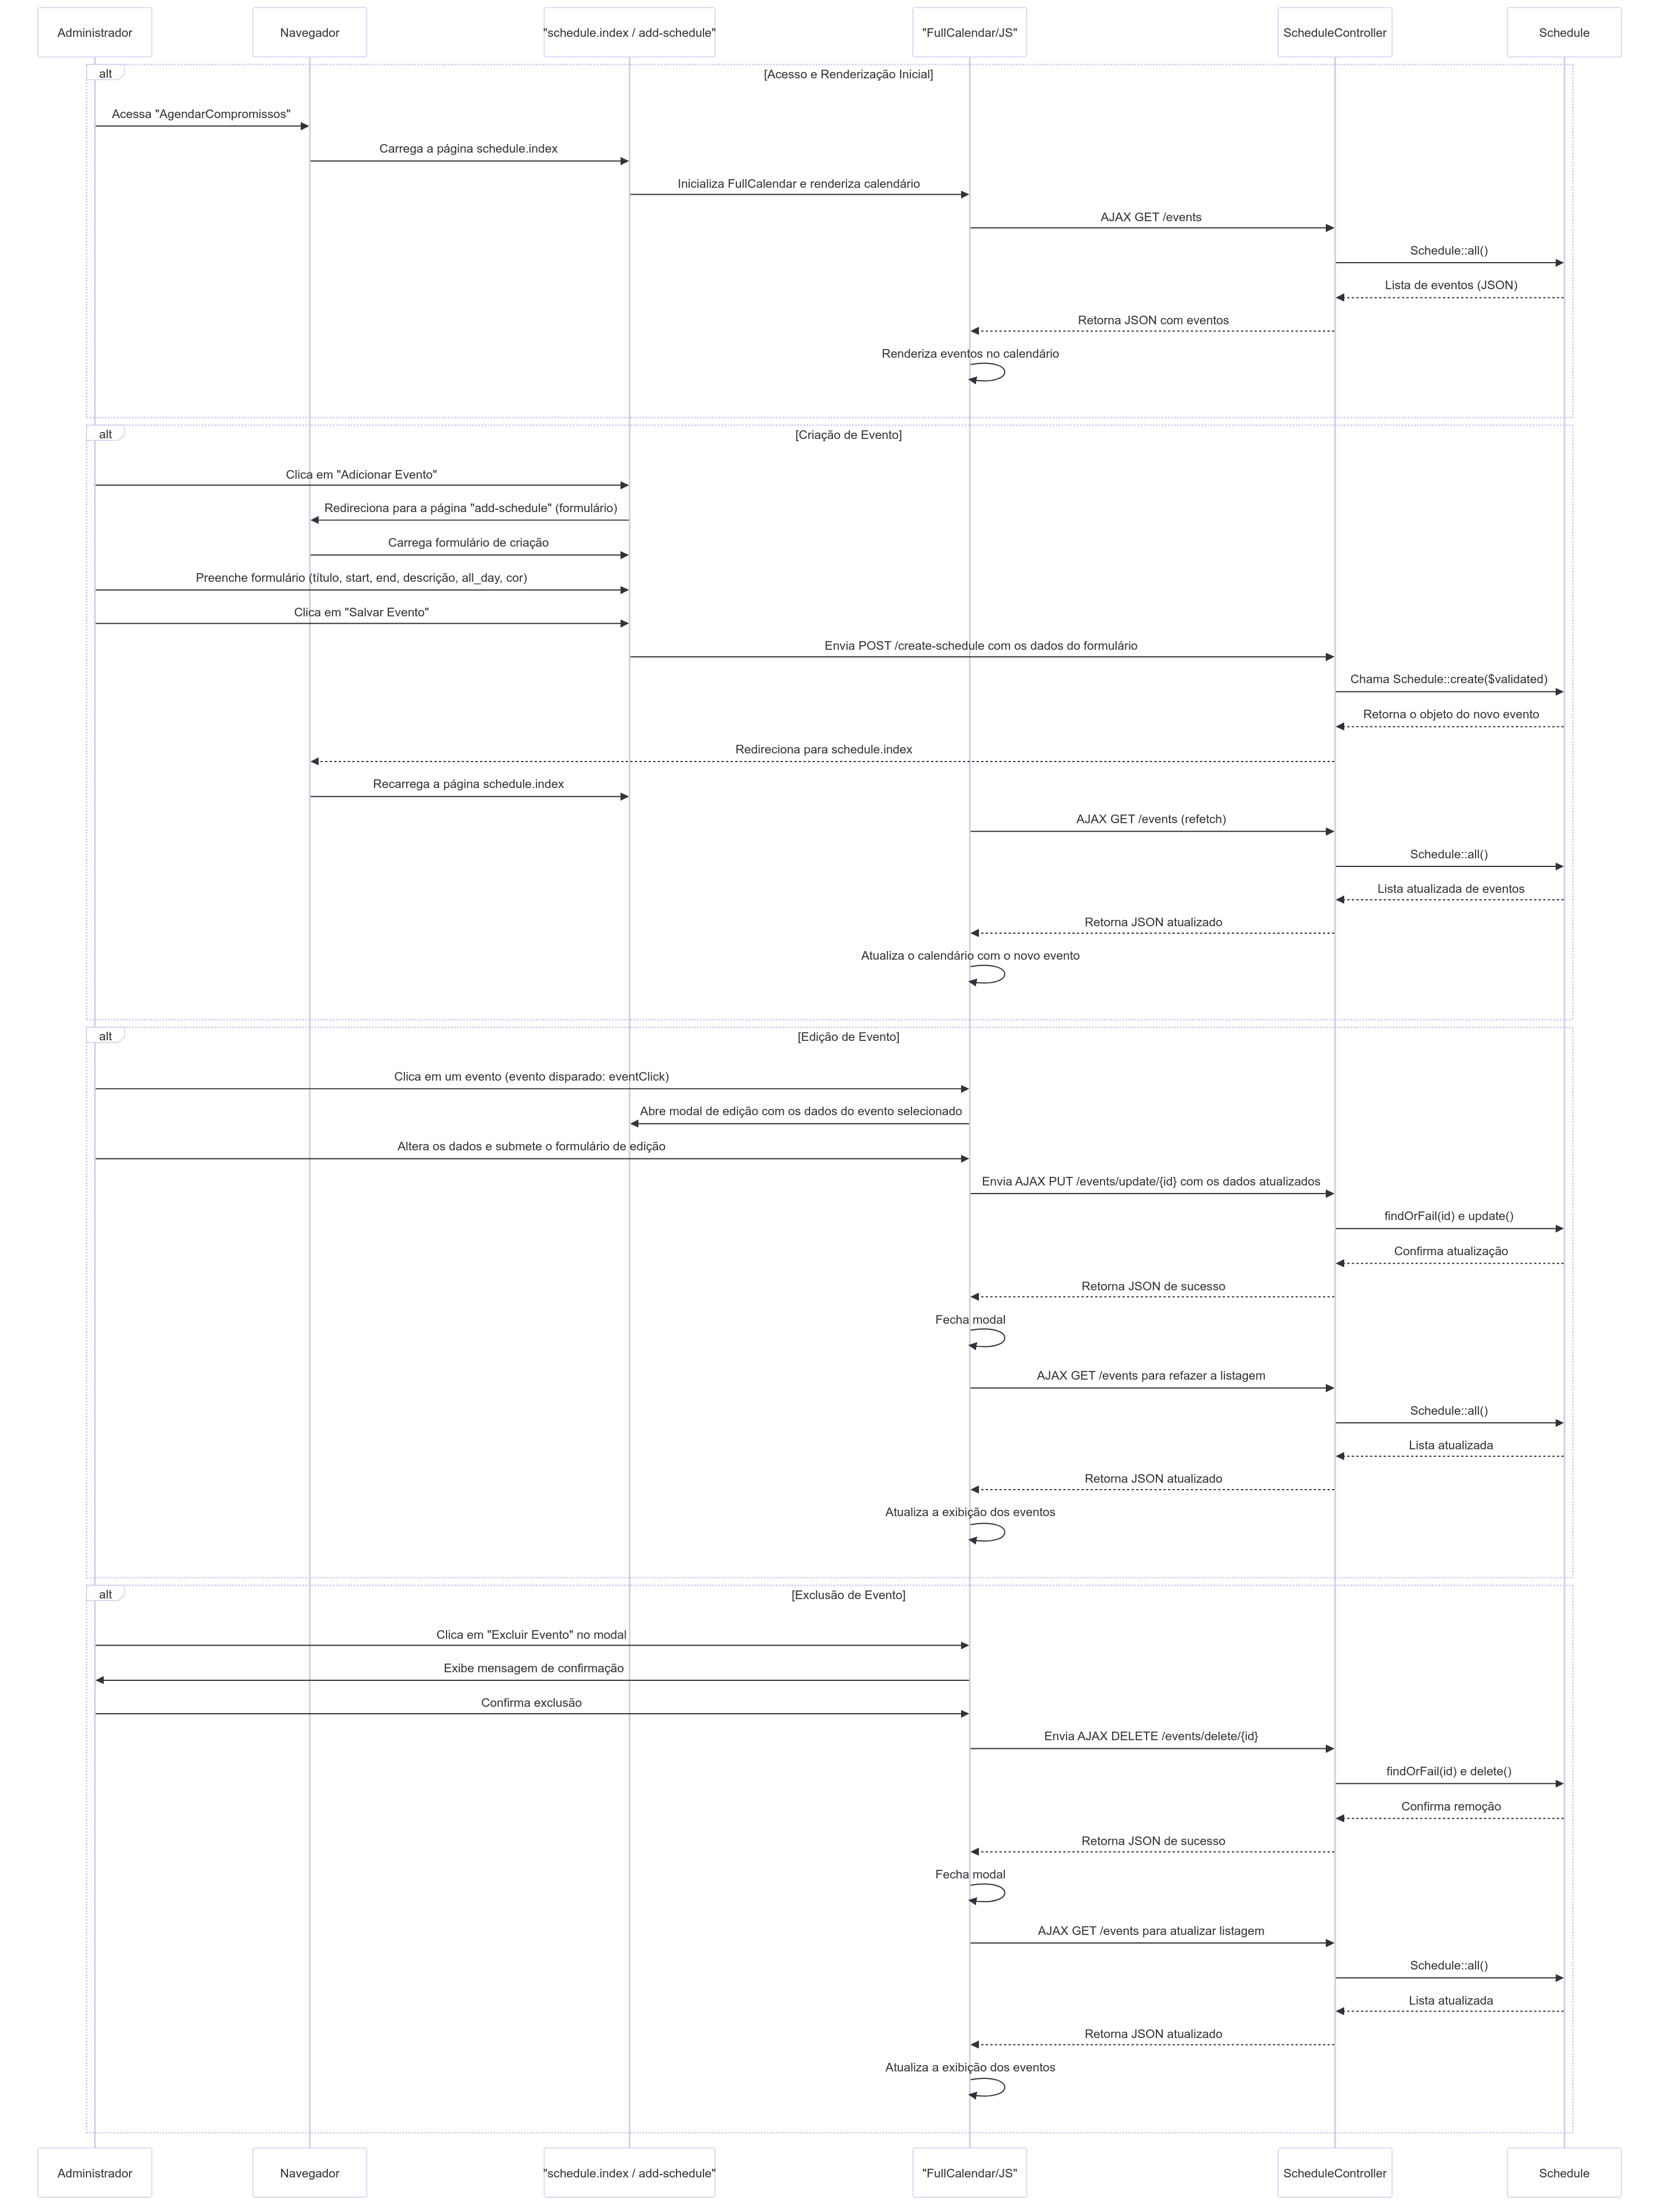
\includegraphics[width=0.8\linewidth]{imagens/uml/Diagrama de sequencia gerenciar eventos (1).png}
\end{figure}

\begin{figure}[!ht]
    \centering
    \caption{Diagrama de Sequencia Marcar Consulta}
    \label{fig:20}
    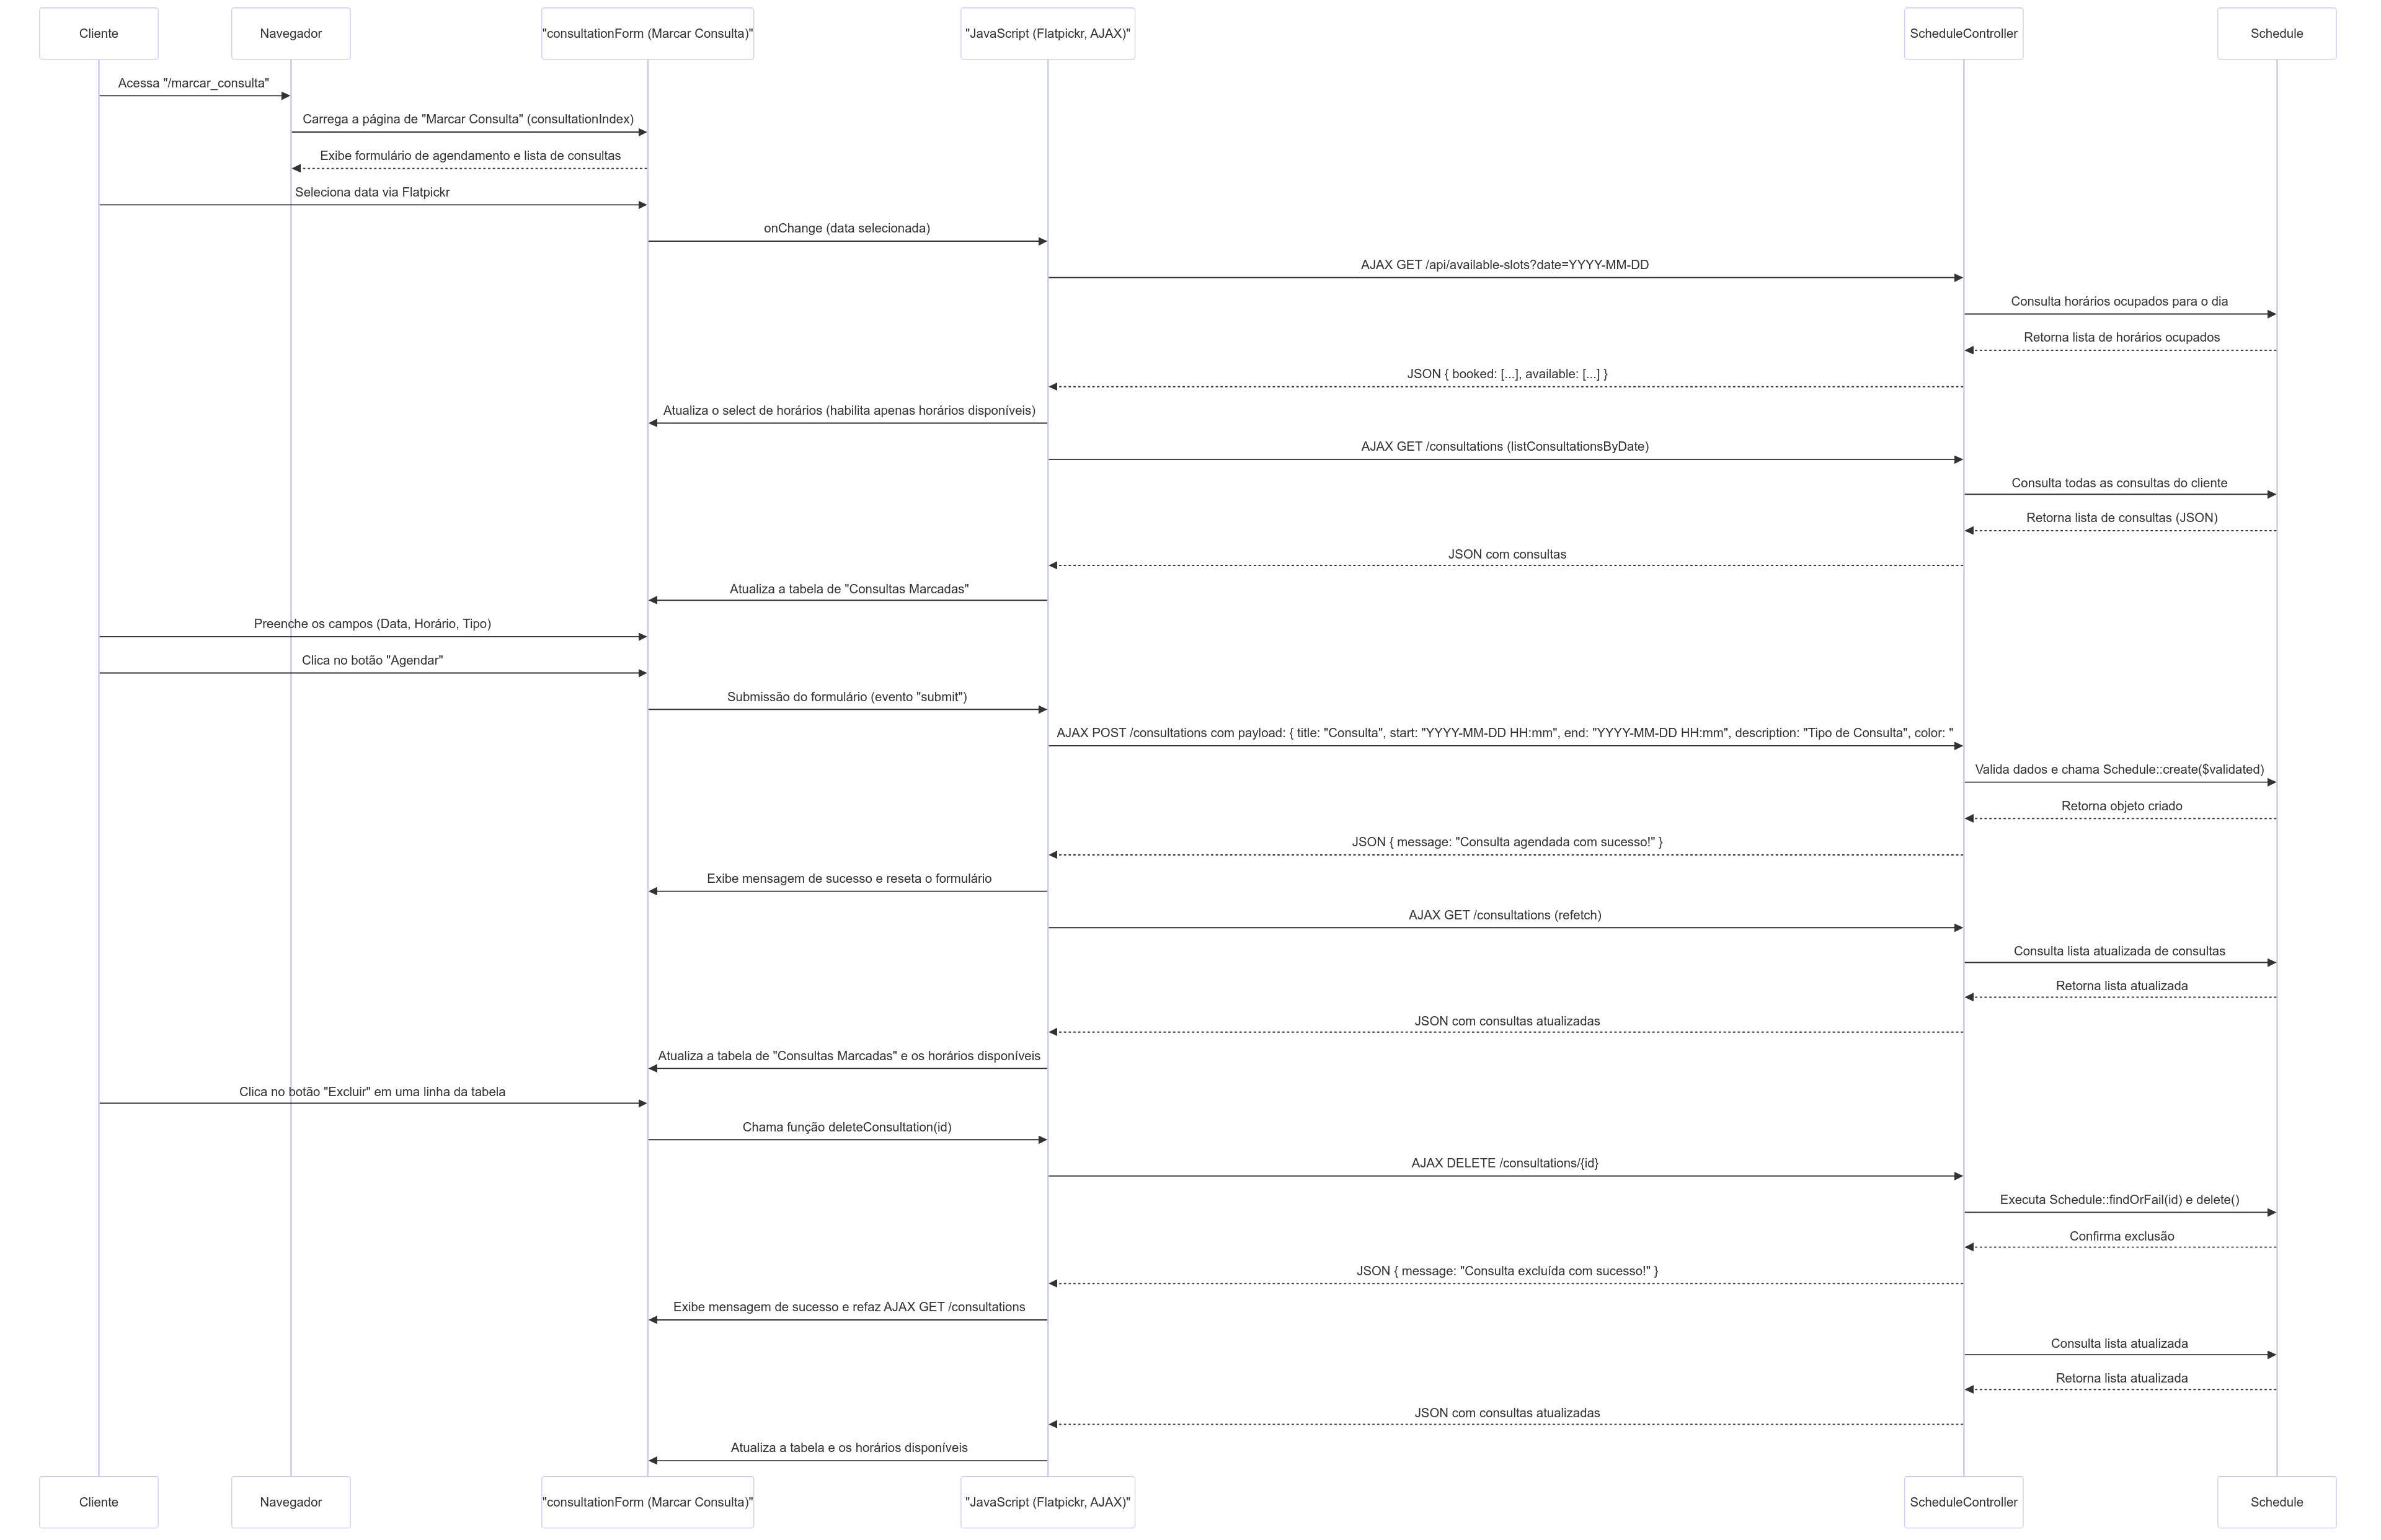
\includegraphics[width=0.8\linewidth]{imagens/uml/Diagrama de sequencia Marcar consulta (1).png}
\end{figure}

\begin{figure}[!ht]
    \centering
    \caption{Diagrama de Sequencia Gerenciar Pagamento}
    \label{fig:21}
    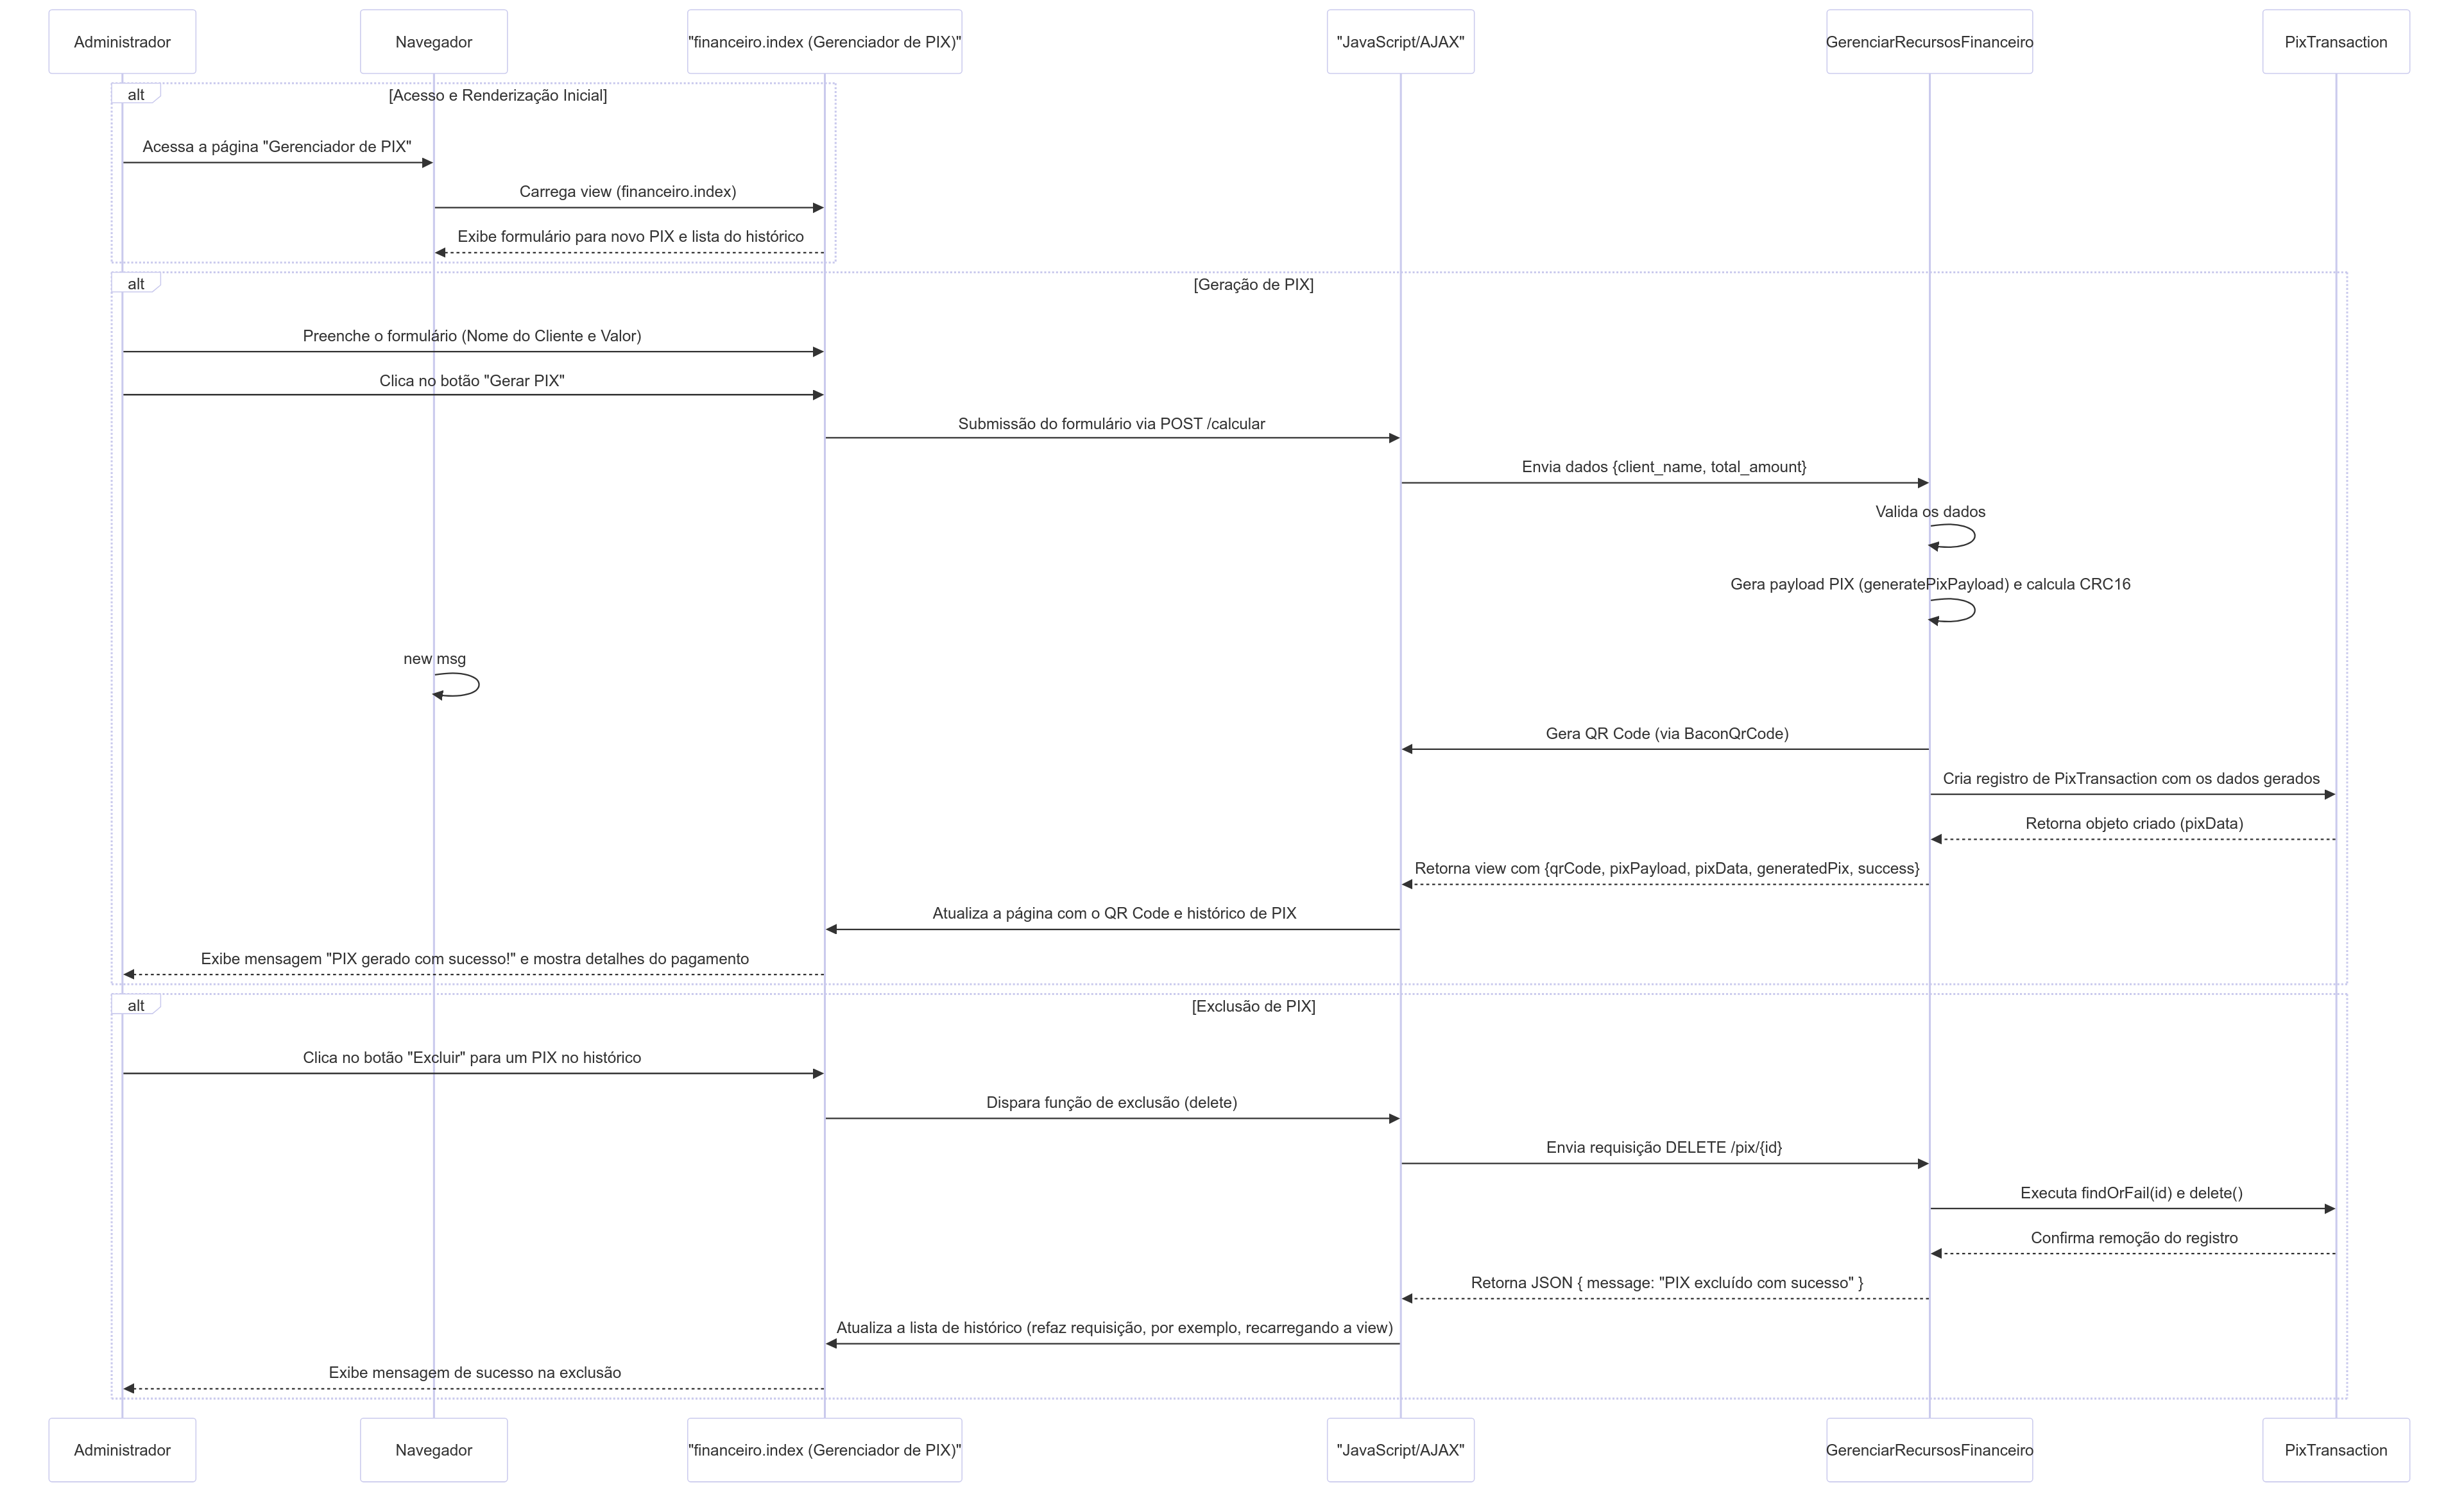
\includegraphics[width=0.8\linewidth]{imagens/uml/Diagrama de sequencia gerenciar Pagamento.png}
\end{figure}

\begin{figure}[!ht]
    \centering
    \caption{Diagrama de Sequencia Processar Pagamento}
    \label{fig:22}
    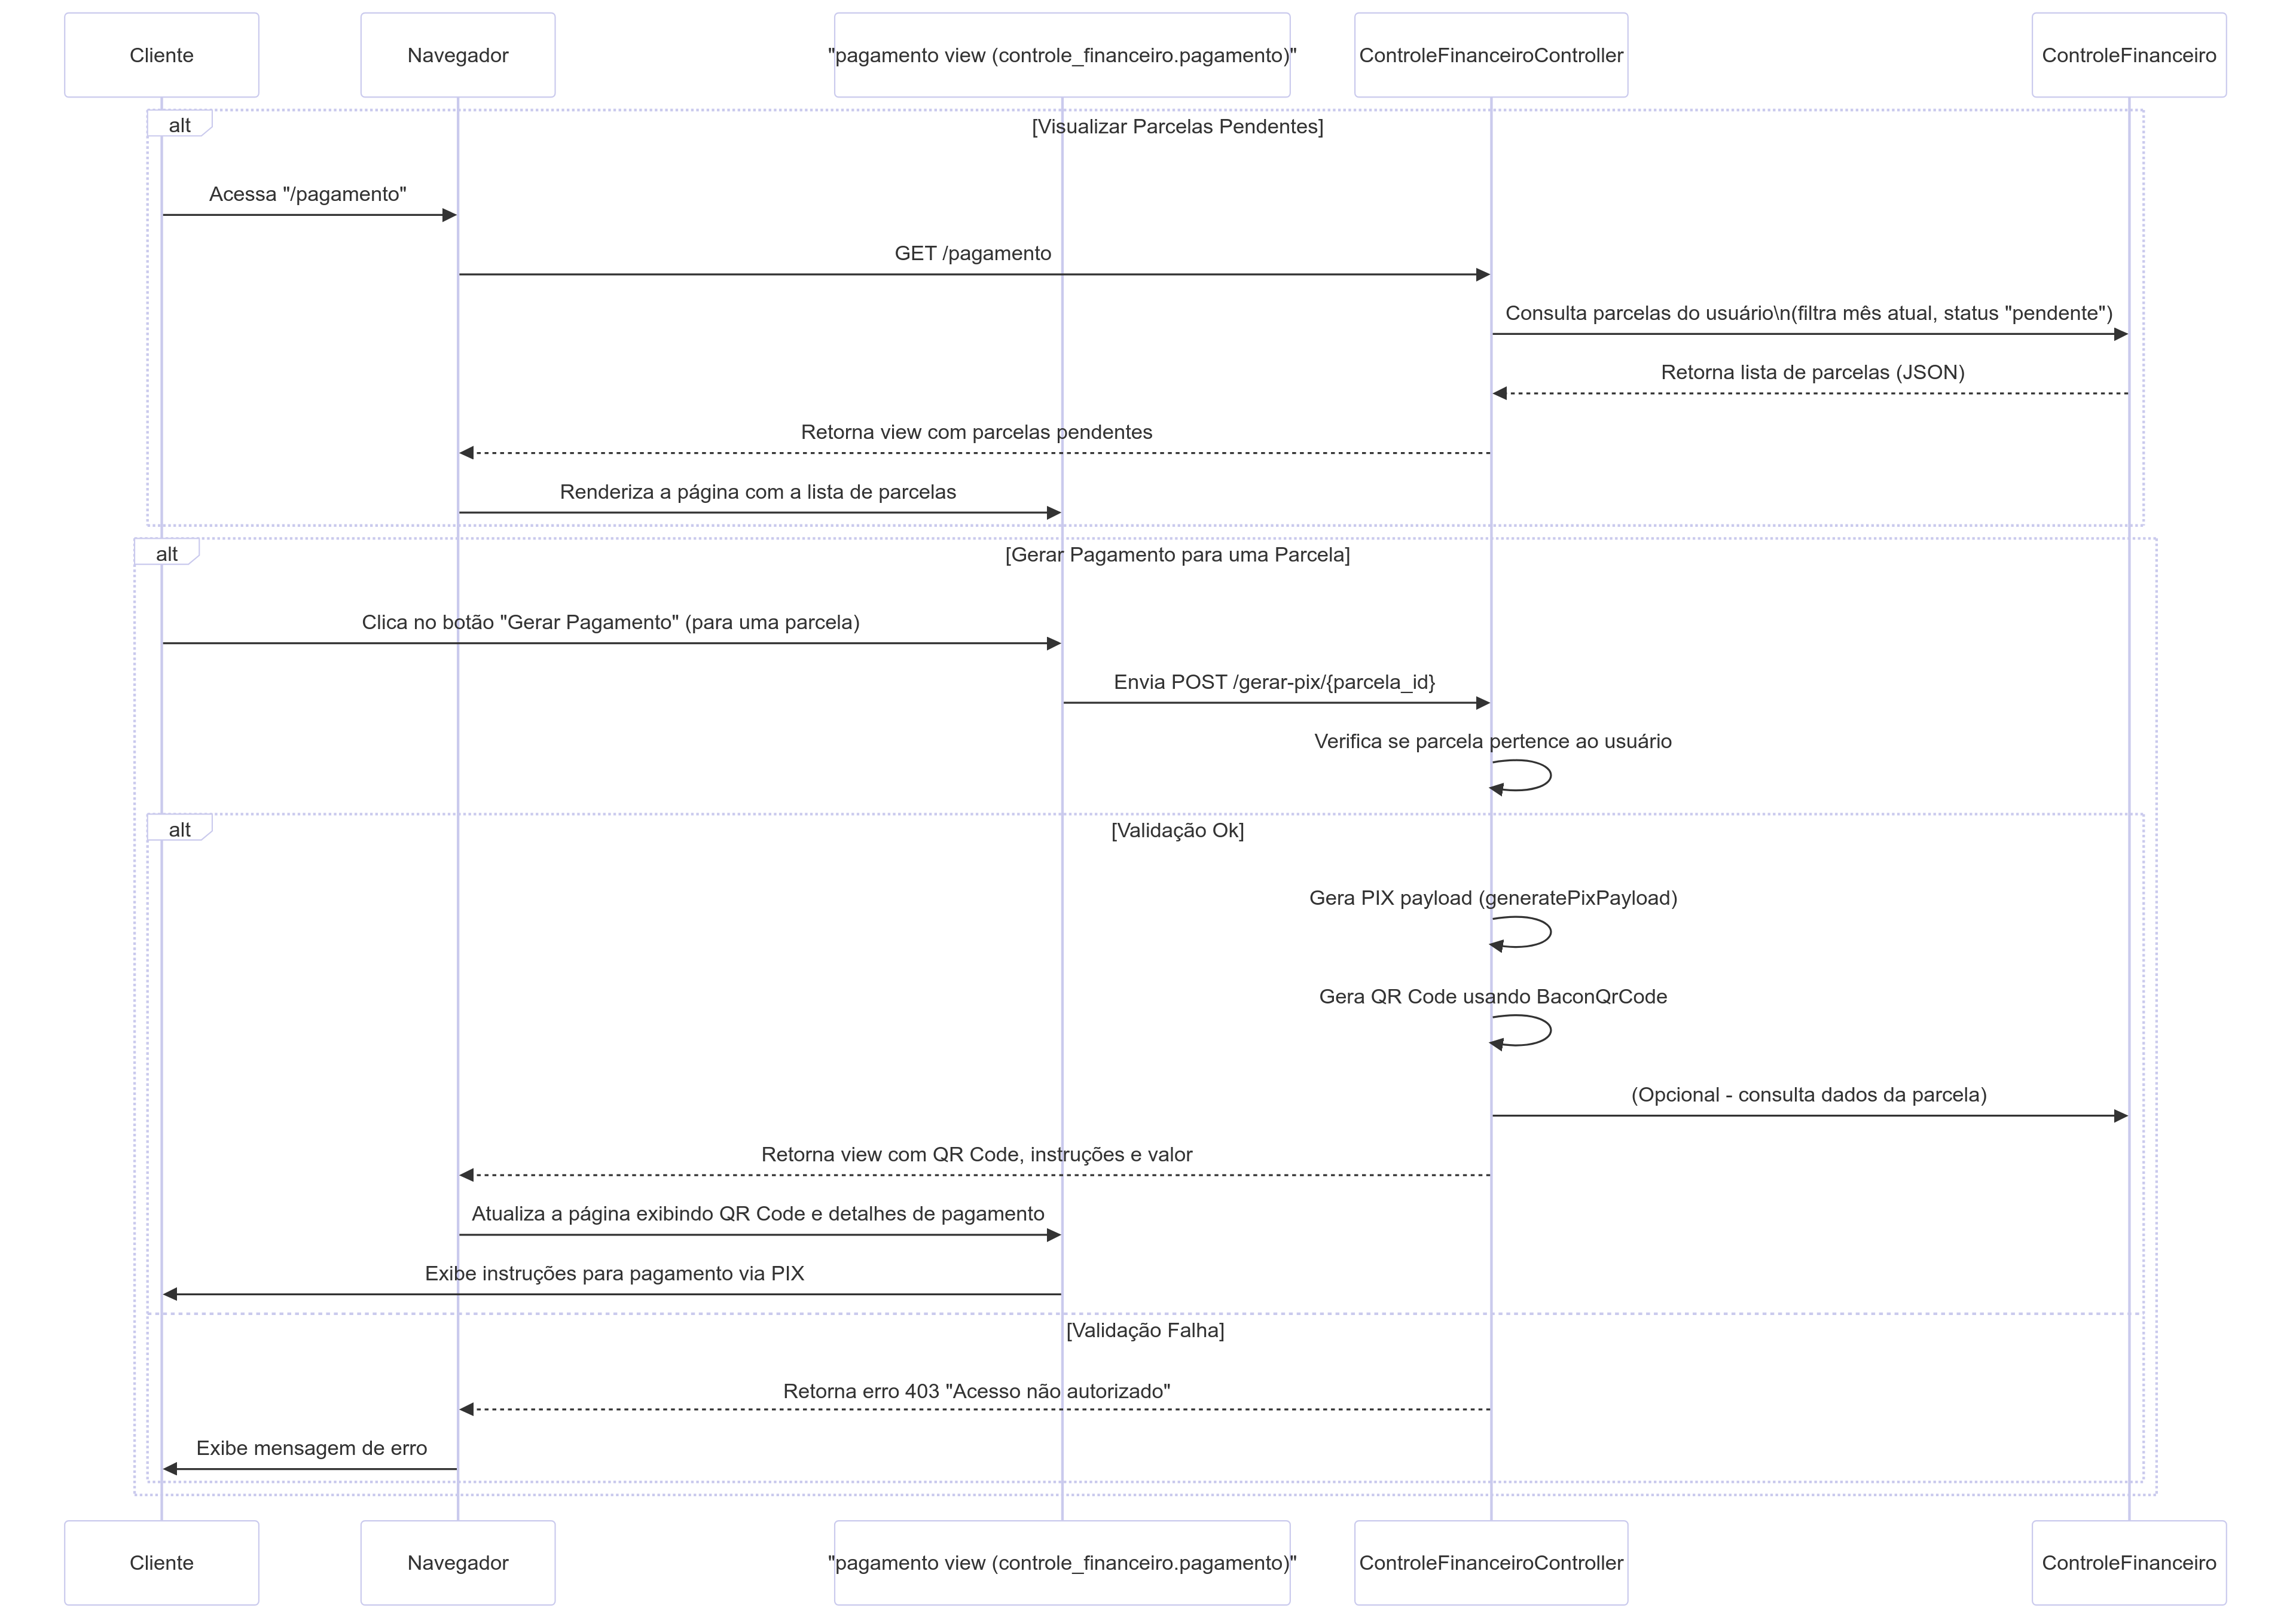
\includegraphics[width=0.8\linewidth]{imagens/uml/Diagrama de sequencia ProcessarPagamento (1).png}
\end{figure}

\begin{figure}[!ht]
    \centering
    \caption{Diagrama de Sequencia Acompanhar Processo Jurídico}
    \label{fig:23}
    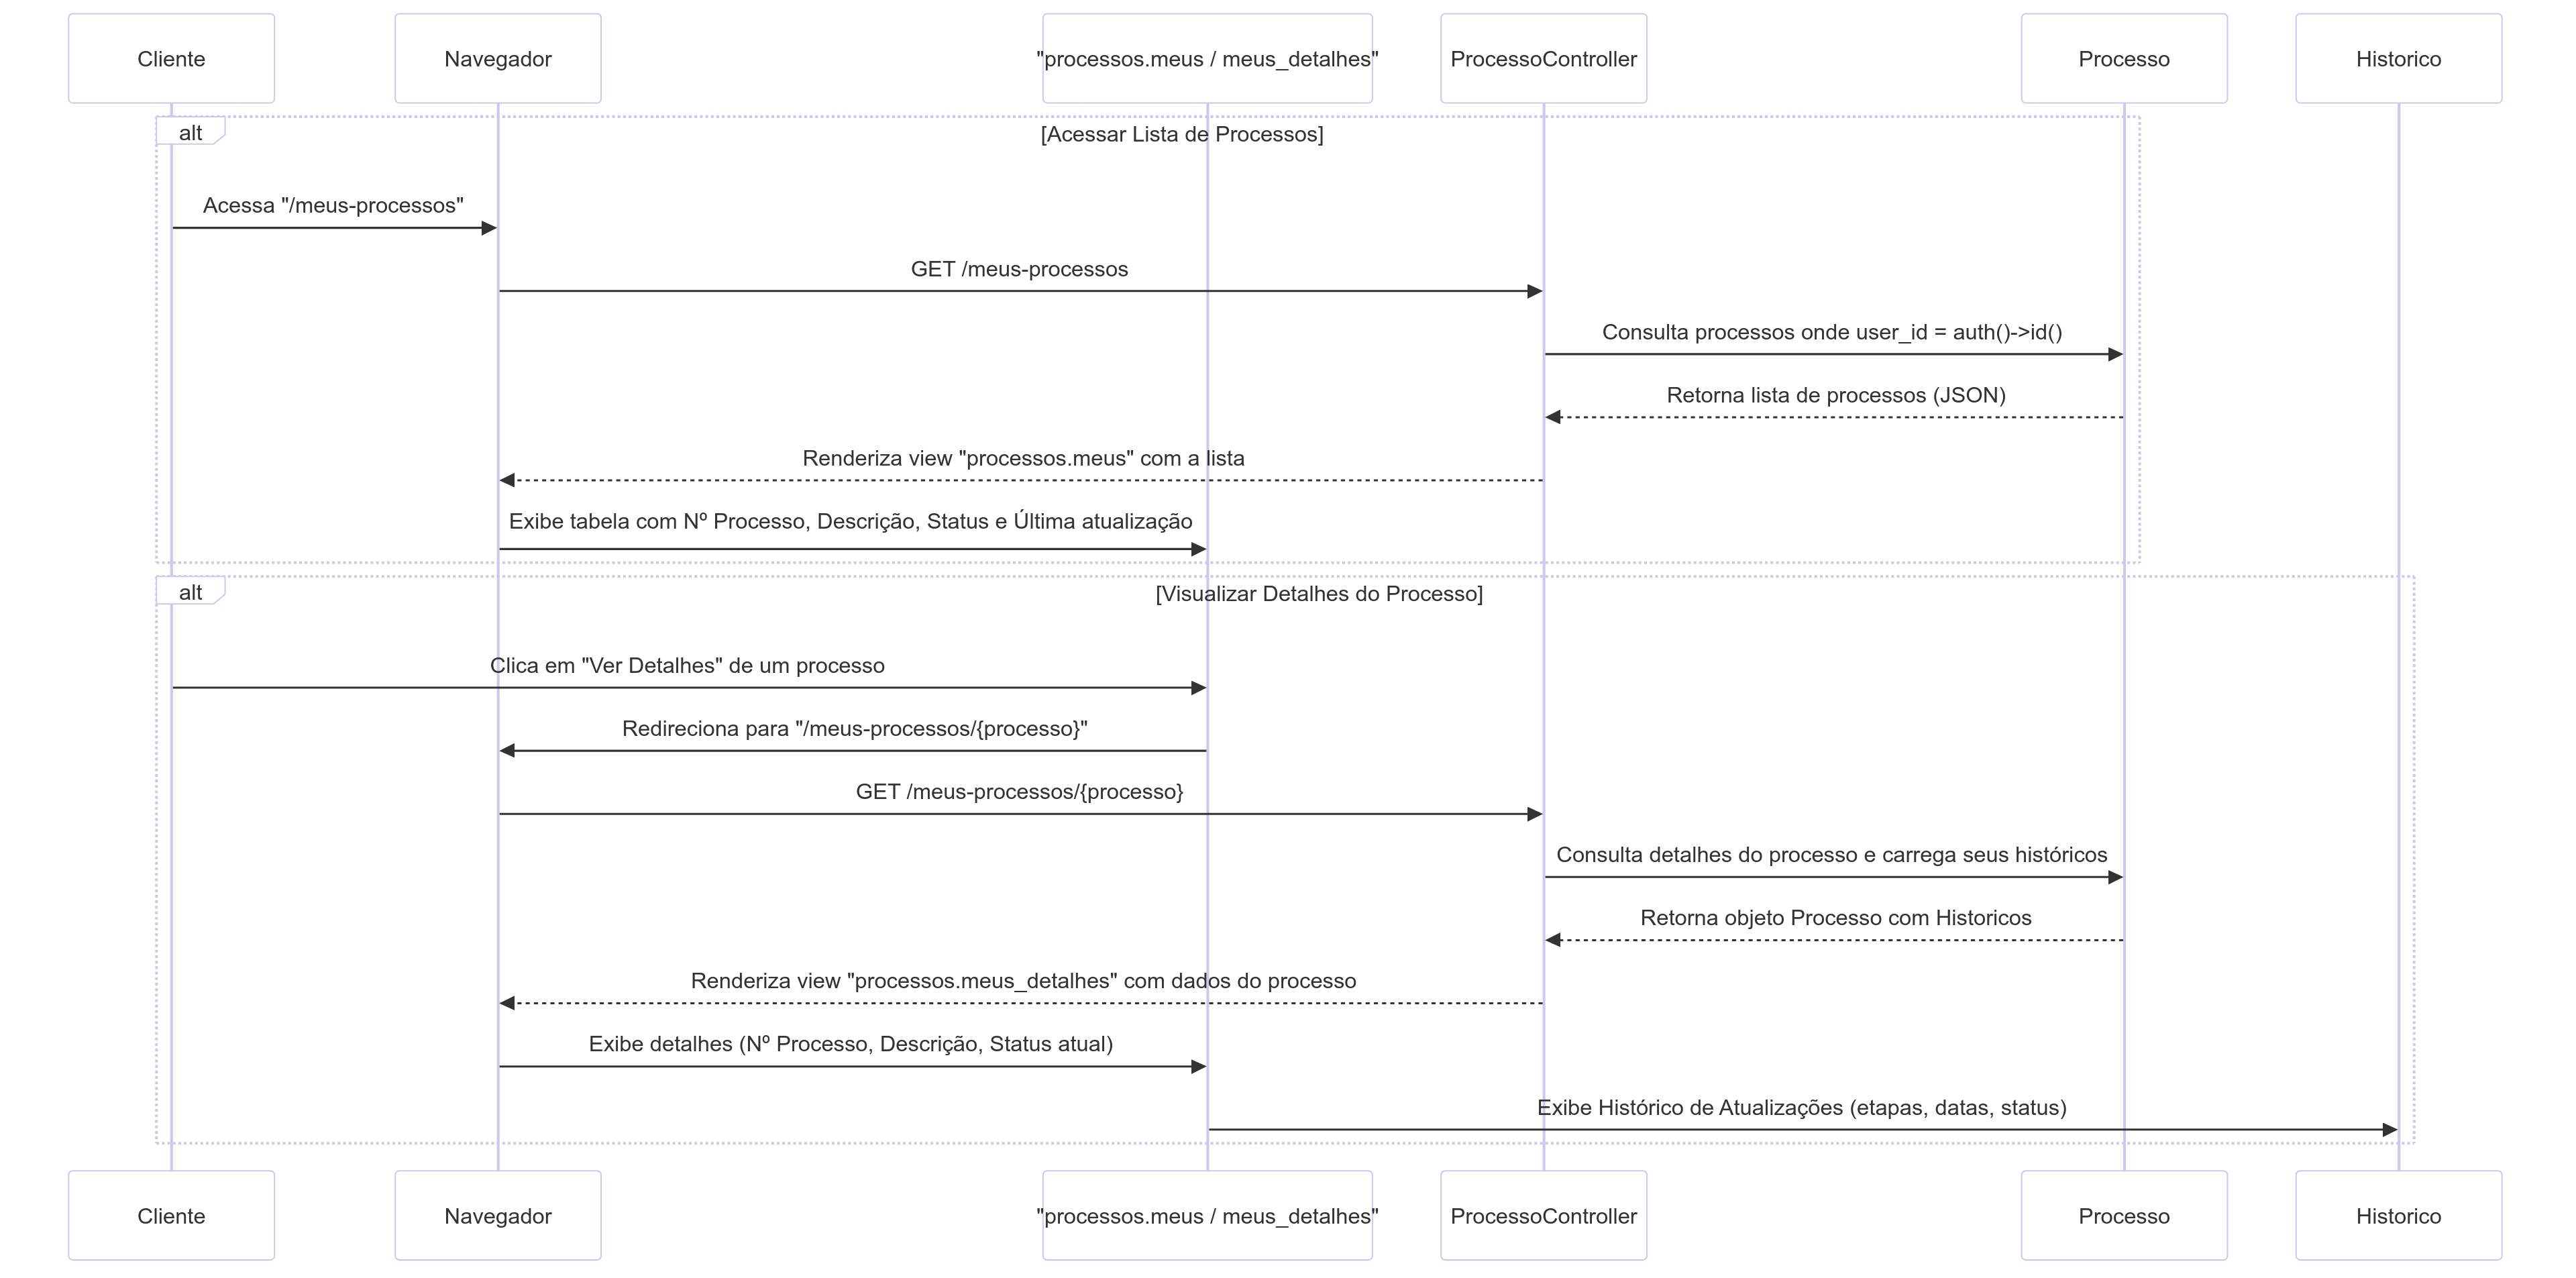
\includegraphics[width=0.8\linewidth]{imagens/uml/Diagrama de sequencia acompanhar processo juridico (1).png}
\end{figure}

\begin{figure}[!ht]
    \centering
    \caption{Diagrama de Sequencia Gerenciar Processo Jurídico}
    \label{fig:24}
    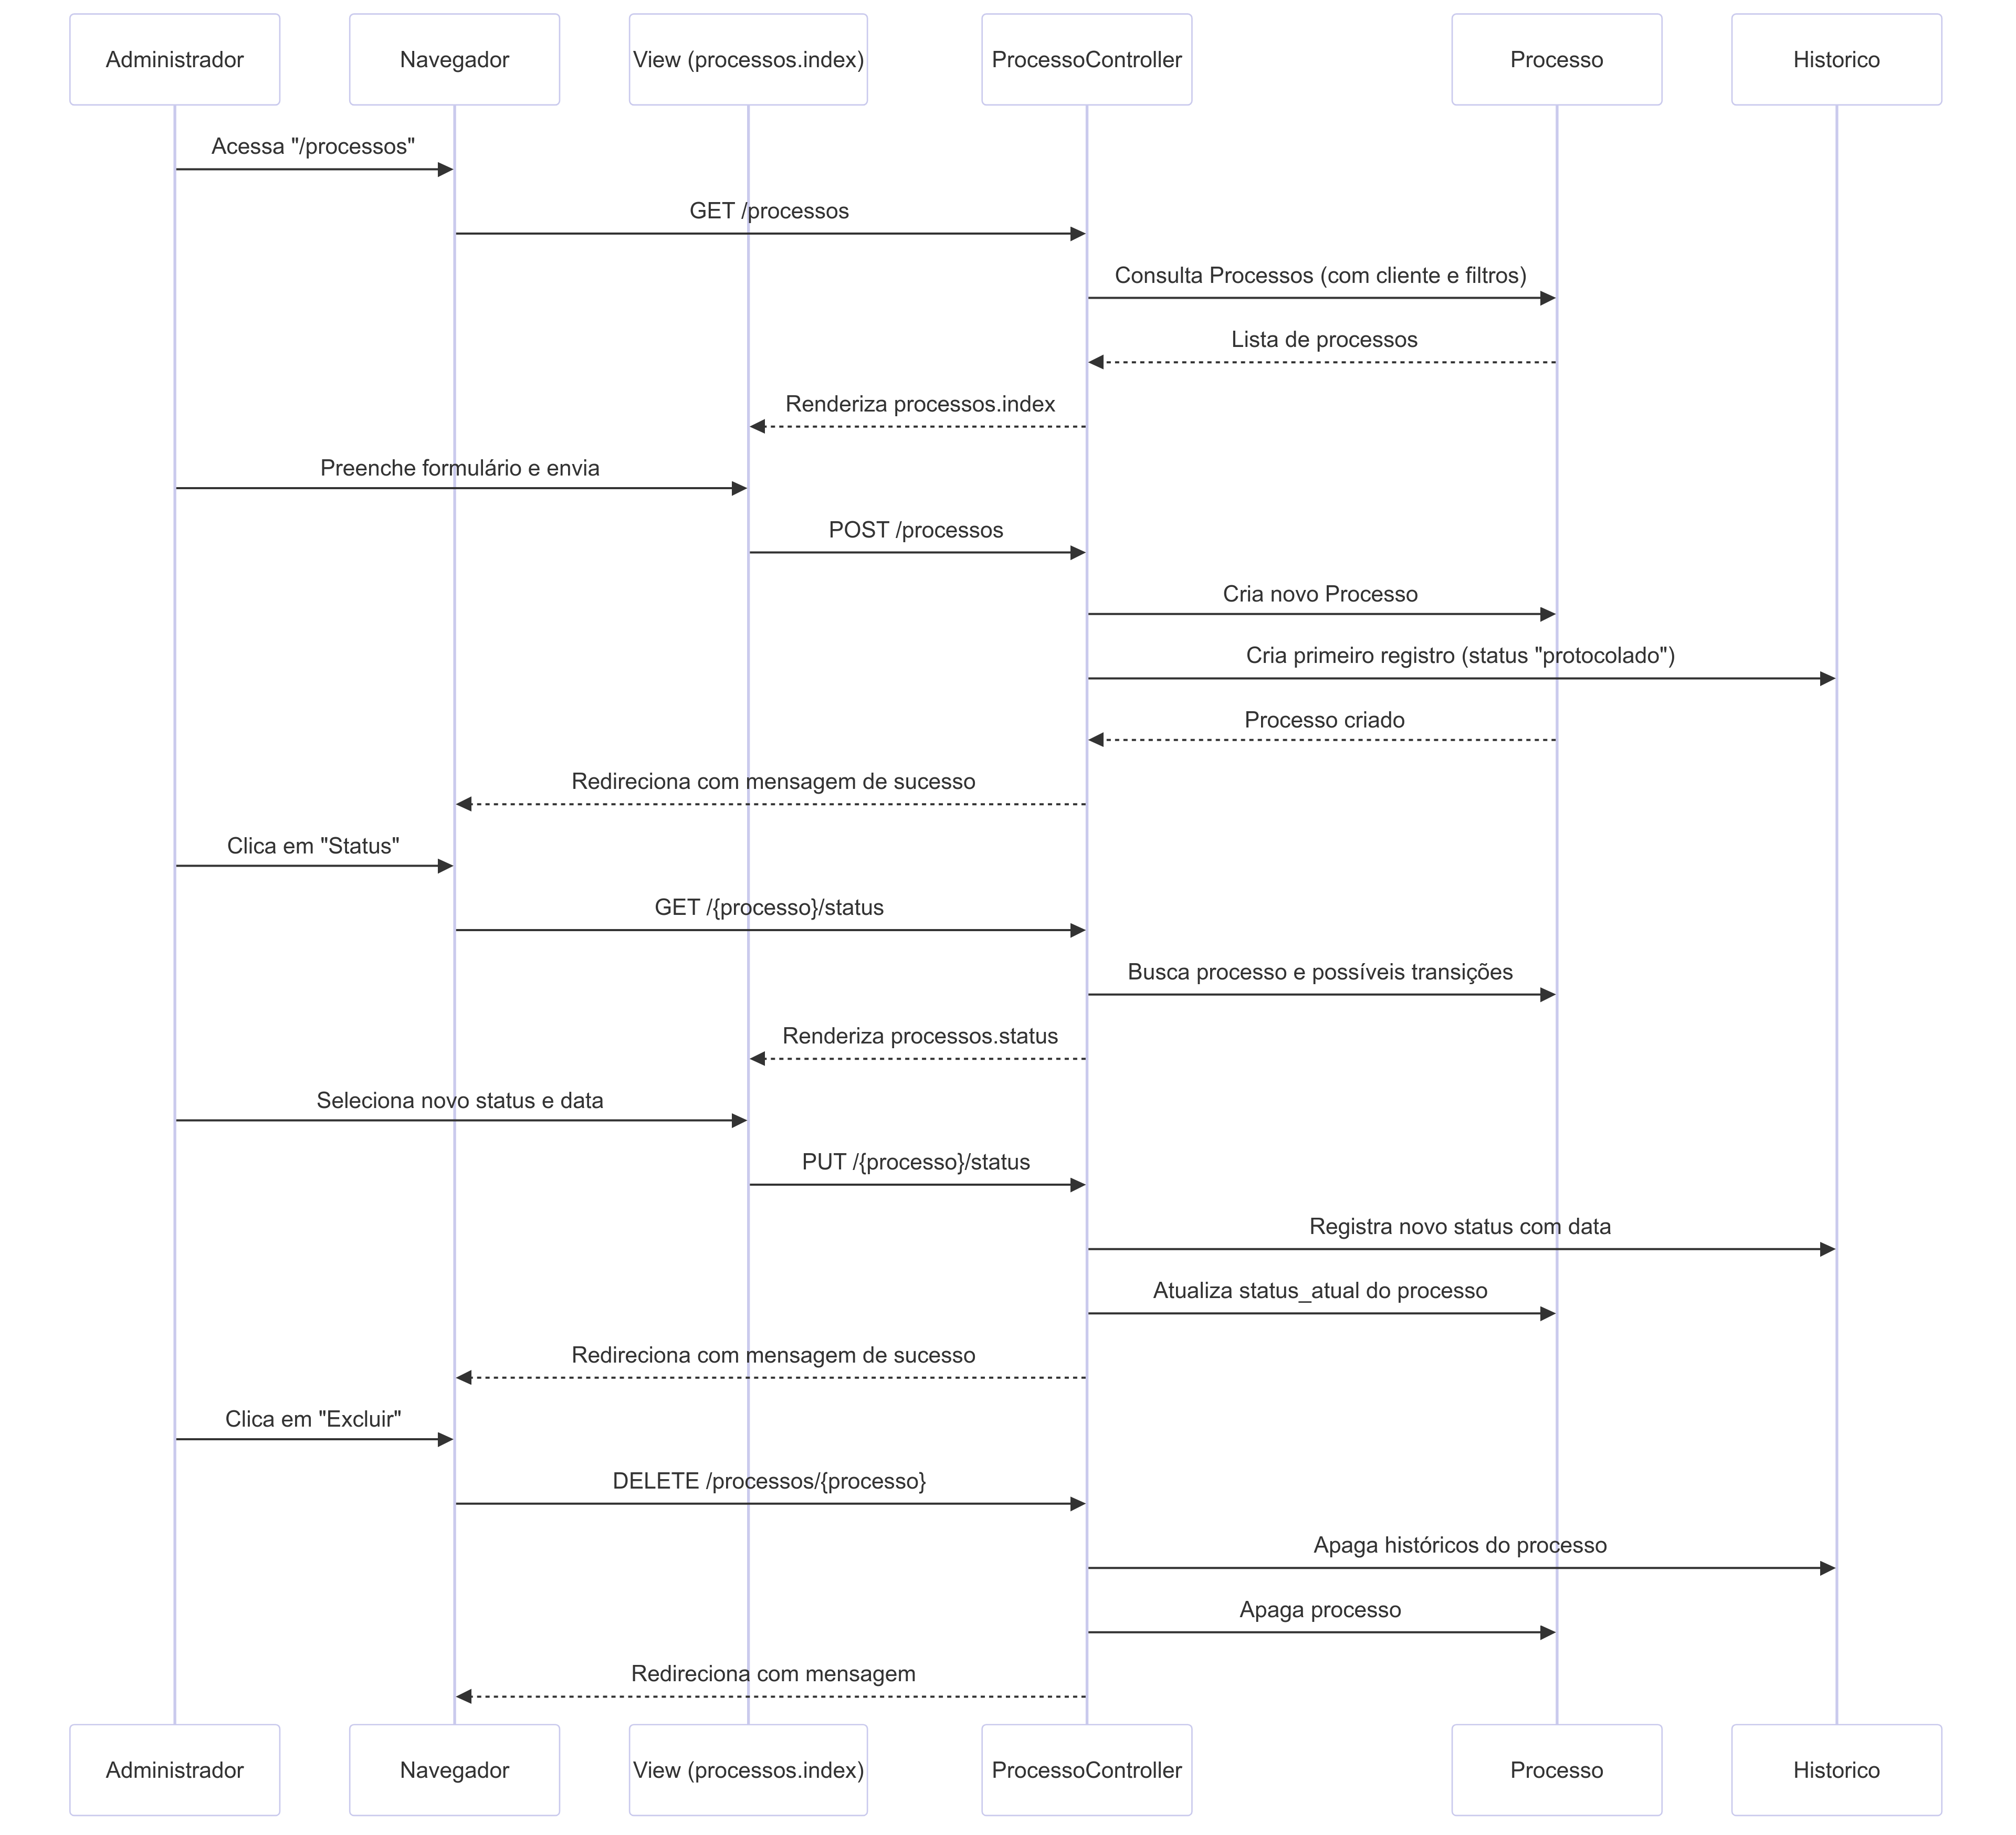
\includegraphics[width=0.8\linewidth]{imagens/uml/Diagrama de sequencia gerenciar processo juridico (1).png}
\end{figure}